\documentclass[12pt,a4paper]{article}
\usepackage{ctex}
\usepackage{graphicx}
\usepackage{geometry}
\usepackage{array}
\usepackage{setspace}
\usepackage{xeCJK}
\usepackage{indentfirst}
\usepackage{amsmath}
\usepackage{amsthm}
\usepackage{float}
\usepackage{subfigure}
\usepackage{booktabs}
\usepackage{multirow}
\usepackage{caption}
\usepackage{listings}
\usepackage{xcolor}
\usepackage{matlab-prettifier}
\usepackage{enumitem}
\captionsetup[table]{position=bottom}

% 页边距
\geometry{left=2.5cm,right=2.5cm,top=2.5cm,bottom=2.5cm}
% 默认宋体小四
\setCJKmainfont[BoldFont=SimHei]{SimSun}
\zihao{-4}
\linespread{1.25}

\lstdefinestyle{Matlab-boxed}{
  style=Matlab-editor,
  frame=single,
  framerule=0.6pt,
  rulecolor=\color{black},
  framesep=6pt,
  backgroundcolor=\color{black!2},
}

\begin{document}
% 实验名称（小二黑体、居中）
\begin{center}
  {\zihao{2}\heiti 核磁共振实验}
\end{center}
% 年级 专业 姓名 座位号（宋体小四、居中、段前后 0.5 行）
\vspace{0.1\baselineskip}
\begin{center}
  （\textbf{年级}\ \underline{2024 级}\quad \textbf{专业}\ \underline{x} \quad \textbf{姓名}\ \underline{Pinco Li} \quad \textbf{座位号} \ \underline{5}）
\end{center}
\vspace{0.1\baselineskip}

\section{实验目的}

\begin{enumerate}
  \item 掌握核磁共振的基本原理和稳态核磁共振技术
  \item 学习利用核磁共振校准磁场
  \item 学习测量 $^1$H 核的基本核参数
  \item 了解核磁共振在各学科的应用
\end{enumerate}

\section{实验仪器}

\begin{figure}[H]
    \centering
    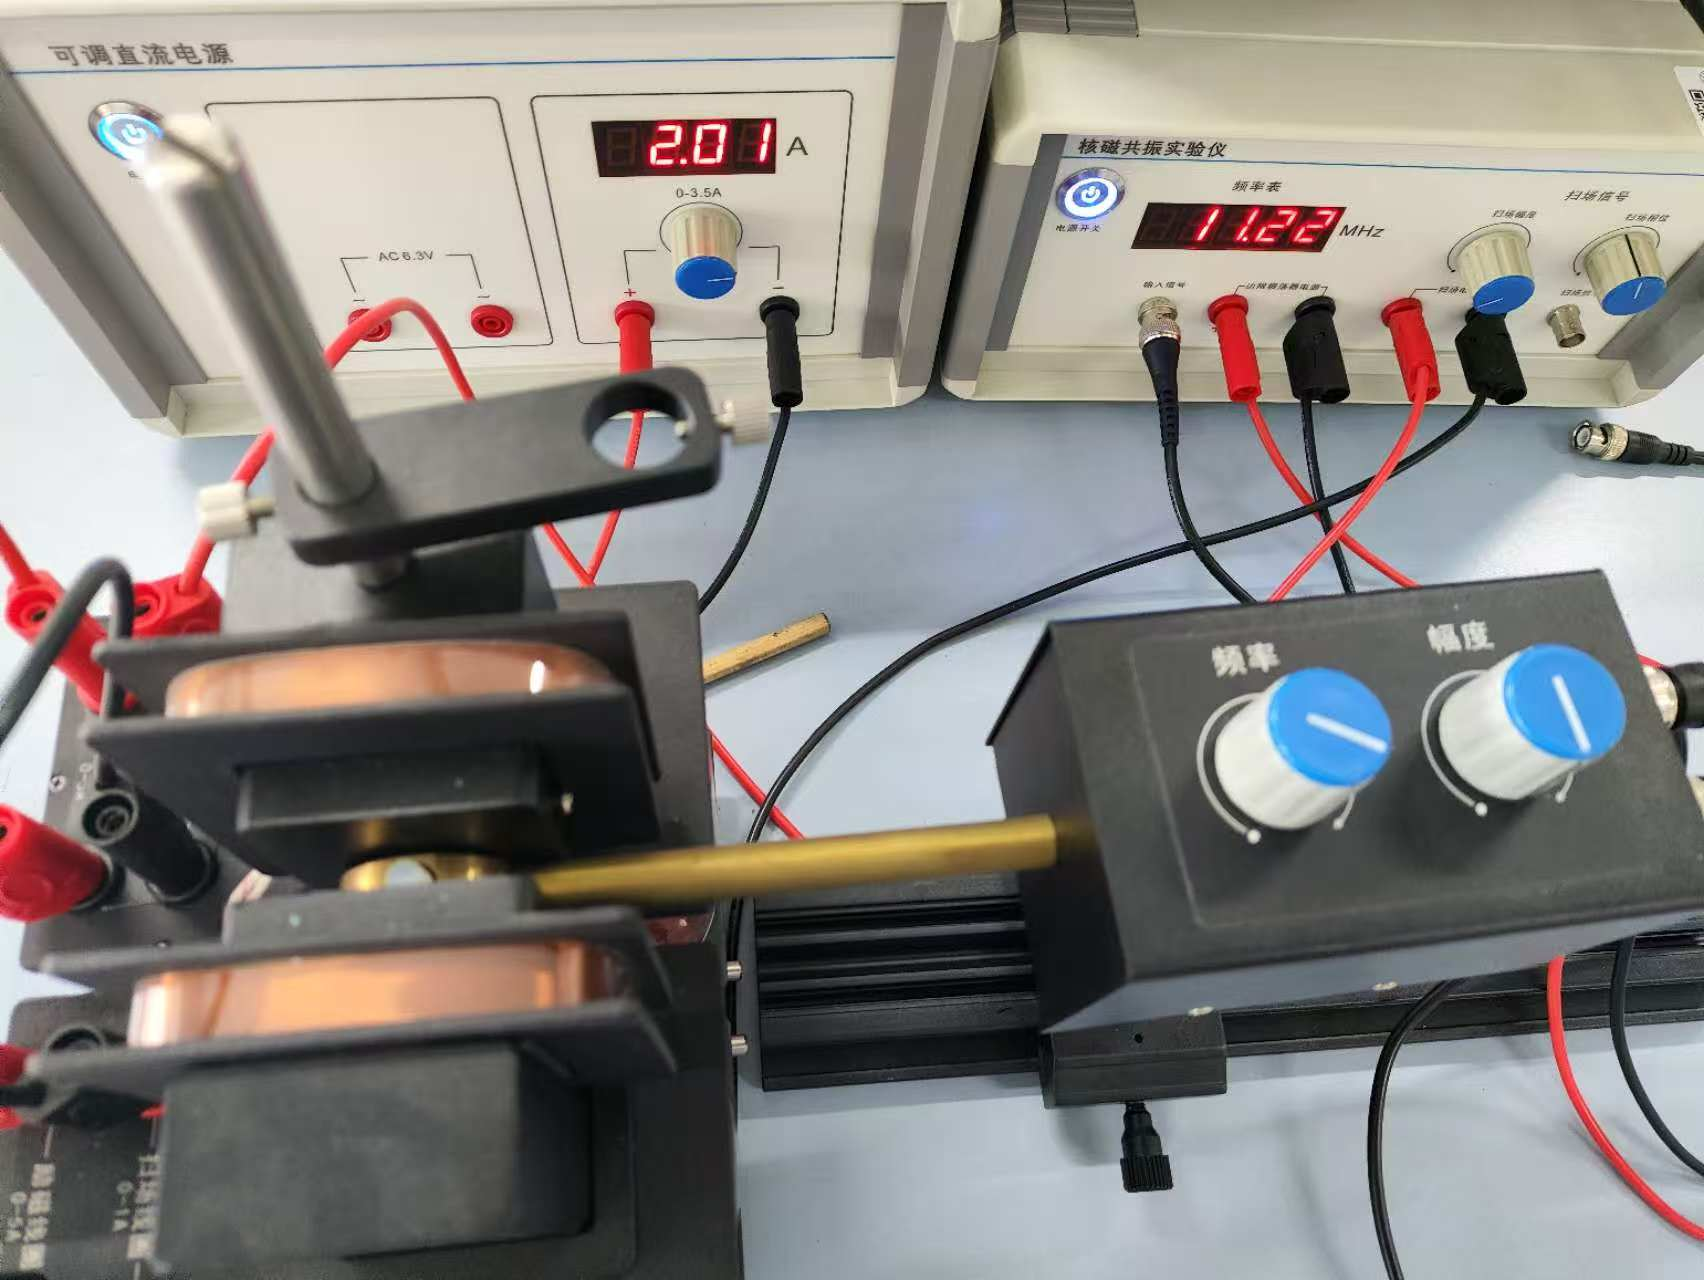
\includegraphics[width=0.6\textwidth]{assets/实验装置.jpg}
    \caption{核磁共振实验装置示意图}
    \label{fig:apparatus}
\end{figure}

\begin{enumerate}
    \item 核磁共振实验仪（型号：CQC-HC03）
    \item 核磁共振探测单元（含探测线圈和样品腔）
    \item U型磁场线圈（含扫场线圈）
    \item 可调直流电源（0-3.5A）
    \item 数字示波器（KEYSIGHT DSOX1202A）
    \item 水样品（硫酸铜溶液CuSO$_4$）和聚四氟乙烯样品（C$_2$F$_4$）
    \item 连接导线若干
\end{enumerate}

\section{实验原理}

\subsection{核磁共振的基本概念}

核磁共振是指具有固定磁矩的原子核在恒定磁场与交变磁场的共同作用下，自旋核吸收特定频率的电磁波，从较低能级跃迁到较高能级，与交变磁场发生能量交换的现象。核磁共振信号实际上是发射出的电磁辐射的物理现象，其强度与核密度成一定比例关系。因此，核磁共振信号可以用来反映样品的化学结构、分子或原子的扩散系数、反应速率、化学变化以及其他性质。这使得核磁共振成为现代科学研究中极为重要的分析手段。

\begin{figure}[H]
    \centering
    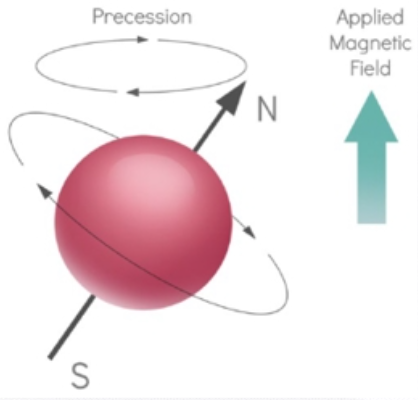
\includegraphics[width=0.3\textwidth]{assets/proton_spin.png}
    \caption{质子在磁场B中的自旋示意}
    \label{fig:proton_spin}
\end{figure}

对于自旋量子数$I \neq 0$的原子核，都具有自旋现象。其自旋角动量$P$可以表示为：
\begin{align}
P = \frac{h}{2\pi}\sqrt{I(I+1)}
\end{align}
其中$h$为普朗克常数。具有自旋角动量的原子核必然具有相应的磁矩$\mu$，磁矩与自旋角动量的关系为：
\begin{align}
\mu = \gamma P
\end{align}
其中$\gamma$称为磁旋比，对于同一种原子核，$\gamma$为一常数。例如对于$^1$H核，$\gamma = 26.752 \times 10^7$ rad·T$^{-1}$·s$^{-1}$；对于$^{13}$C核，$\gamma = 6.728 \times 10^7$ rad·T$^{-1}$·s$^{-1}$；对于$^{19}$F核，$\gamma = 25.181 \times 10^7$ rad·T$^{-1}$·s$^{-1}$。

\subsection{能级分裂与共振条件}

对于自旋量子数$I=1/2$的原子核，在外加磁场中只有$m=+1/2$和$m=-1/2$两种取向。当$m=+1/2$时，原子核与外磁场顺向排列，能量较低；当$m=-1/2$时，原子核与外磁场逆向排列，能量较高。这两个能级的能量分别为：
\begin{align}
E_{1/2} &= -\gamma \frac{h}{2\pi}\left(+\frac{1}{2}\right)B\\
E_{-1/2} &= -\gamma \frac{h}{2\pi}\left(-\frac{1}{2}\right)B
\end{align}

\begin{figure}[H]
    \centering
    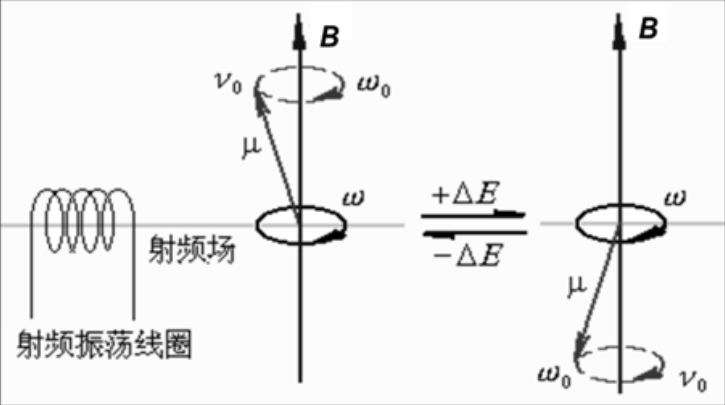
\includegraphics[width=0.6\textwidth]{assets/magnetic_interaction.png}
    \caption{外加磁场中电磁辐射与进动核的相互作用示意}
    \label{fig:magnetic_interaction}
\end{figure}

根据量子力学的选择定则，只有$\Delta m = \pm1$的跃迁才是允许的。因此相邻能级之间的能量差为：
\begin{align}
\Delta E = \gamma \frac{h}{2\pi} B
\end{align}

若在垂直于恒定磁场$B$的方向上施加一个射频场，其频率为$\nu_1$，当$\nu_1=\nu_0$时，自旋核会吸收射频的能量，由低能态跃迁到高能态，这种现象称为核磁共振吸收。根据能量守恒定律，共振条件可以表示为：
\begin{align}
\Delta E = h \nu
\end{align}

由此可得共振频率与磁场强度的关系：
\begin{align}
\nu = \frac{\gamma}{2\pi} B
\end{align}

对于同一种原子核，$\gamma$为常数，磁场$B$越强，共振频率$\nu$越大。对于裸露的$^1$H核而言，经过大量测量得到：
\begin{align}
\frac{\gamma}{2\pi} = 42.577469 \text{ MHz/T}
\end{align}

\subsection{化学位移与磁场校准}

需要注意的是，对于原子或分子中处于不同基团的原子，由于不同原子所处的化学环境不同，受到周围电子屏蔽的情况不同，$\frac{\gamma}{2\pi}$的数值将略有差别，共振吸收频率亦不同。这种现象称为化学位移。通过测量质子在磁场中的共振频率$\nu$，可以实现对磁场的校准：
\begin{align}
B = \frac{2\pi}{\gamma}\cdot \nu
\end{align}

反之，若磁场$B$已经校准，通过测量未知原子的共振频率$\nu$便可求出待测原子的$\gamma$值或者g因子。这为精确测定原子核参数提供了有效方法。

\subsection{弛豫过程}

要想保持核磁共振信号的检测，必须要有某种过程使高能态的核以非辐射的形式放出能量回到低能态，重建玻尔兹曼分布，这种过程称为弛豫过程。在核磁共振实验中，弛豫过程对信号的稳定性和可重复性至关重要。

为观察到共振现象，通常有两种方法：一是固定磁场$B$，连续改变射频的频率（frequency-sweep）；二是固定射频场的频率，由Helmholtz线圈连续改变磁场强度，从低场向高场扫描（field-sweep，本实验采用的方法）。如果磁场的变化不是太快，而是缓慢通过与射频$\nu$对应的磁场时，即通过共振区的时间远远比弛豫时间$T_1$和$T_2$长得多时，才能得到具有稳态共振吸收信号。

\section{实验步骤}

\subsection{实验准备与调试}

实验开始前，首先按照要求连接好所有导线，确保电路连接正确无误。小心地将水样品放入探测线圈中，并轻轻推动导轨上的拖板，使探测线圈和样品大致置于磁场的中心位置。由于涉及玻璃元件，在放置样品时需要格外小心，避免损坏。

调节恒流源的励磁电流输出为0A，将核磁共振实验仪的扫场幅度旋钮调到较大幅度，约为总输出的1/3圈左右，即右旋转约半圈。将探测器单元的幅度调节旋钮调到最右边，即顺时针旋到底。此时应可在示波器上看到一个类似正弦波的图形，这是扫场信号。

\subsection{寻找共振信号}

将探测器单元的频率调节旋钮调到较小的数值，例如10.0MHz，频率值显示在实验仪的频率表中。慢慢地调节恒流源的旋钮，增加电磁铁线圈的励磁电流、加大磁场强度，直到在示波器上原来正弦波的基础上看到振荡波形，这就是共振信号。若共振信号太大或太小，可以调节示波器电压增益旋钮进行调整。

\begin{figure}[H]
    \centering
    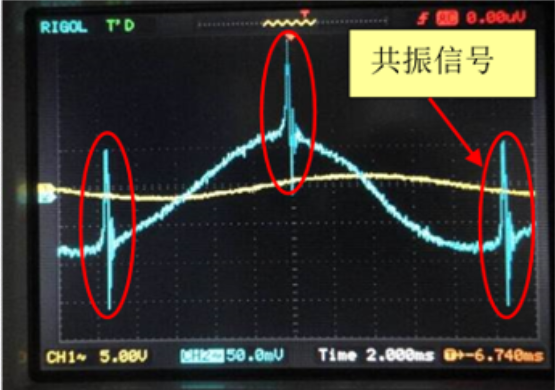
\includegraphics[width=0.6\textwidth]{assets/resonance_signal.png}
    \caption{示波器上观察到的共振信号示意图}
    \label{fig:resonance_signal}
\end{figure}

慢慢地调节实验仪的扫场幅度调节旋钮，可以调小或调大，使共振信号幅度最大。若信号移位或消失，可以微调励磁电流旋钮使其再出现。然后慢慢微调导轨上的拖板和升降调节架，直至样品在磁场中的位置找到共振信号最大的测量位置。最后微调励磁电流大小，使共振信号在示波器横轴方向上均匀分布，即几个信号在示波器x轴方向上等间距排列。

\subsection{数据测量}

将水样品放入探测线圈中，重复前面步骤，找到最佳共振信号。调节频率旋钮或者改变励磁电流大小，使示波器上每个共振信号的时间间隔一样。对照仪器编号，用电流对照表查出此时磁场的$B_0$值，读出核磁共振实验仪表上频率计的显示频率$\nu$，把它们记录在表中。

增加频率$\nu$，例如每次增加0.3 MHz左右，调节励磁电流大小，使示波器上又一次出现时间间隔一样的共振信号。记录下磁场强度$B_0$和共振频率$\nu$。重复上述步骤，测量多组数据，以便进行线性拟合分析。完成水样品测量后，更换为聚四氟乙烯样品，重复上述测量过程。

\section{数据记录与处理}

\subsection{电流与磁感应强度标定数据}

本次实验使用的核磁共振实验仪器编号为CQC-HC03-23030909，室温约25℃。根据仪器提供的标定数据，励磁电流与磁感应强度的关系如下表所示：

\begin{table}[H]
\centering
\begin{tabular}{|c|c|}
\hline
励磁电流 $I$ (A) & 磁感应强度 $B$ (T) \\
\hline
1.30 & 0.202 \\
\hline
1.40 & 0.213 \\
\hline
1.50 & 0.224 \\
\hline
1.60 & 0.234 \\
\hline
1.70 & 0.242 \\
\hline
1.80 & 0.249 \\
\hline
1.90 & 0.255 \\
\hline
2.00 & 0.261 \\
\hline
2.10 & 0.265 \\
\hline
2.20 & 0.270 \\
\hline
2.30 & 0.274 \\
\hline
\end{tabular}
\caption{励磁电流与磁感应强度的标定关系}
\end{table}

通过该标定数据，可以建立励磁电流与磁感应强度之间的对应关系，为后续的磁场校准和数据处理提供依据。数据显示，在测量范围内，磁感应强度随励磁电流的增加而近似线性增加，这符合电磁铁的基本特性。

\subsection{水样品核磁共振测量数据}

本实验使用的水样品为硫酸铜溶液（CuSO$_4$），目的是减少水中氢键的影响，使共振信号更加清晰。测量得到的共振频率与励磁电流的对应关系如下表所示。表中的磁感应强度$B_0$是根据前述标定关系，通过线性插值从励磁电流$I$计算得到的，为后续的数据处理和拟合分析提供了准确的磁场强度数据。

\begin{table}[H]
\centering
\begin{tabular}{|c|c|c|c|}
\hline
序号 & 频率 $\nu$ (MHz) & 电流 $I$ (A) & 磁感应强度 $B_0$ (T) \\
\hline
1 & 11.60 & 2.24 & 0.2716 \\
\hline
2 & 11.23 & 2.02 & 0.2618 \\
\hline
3 & 11.18 & 2.00 & 0.2610 \\
\hline
4 & 10.95 & 1.96 & 0.2586 \\
\hline
5 & 10.77 & 1.80 & 0.2490 \\
\hline
6 & 10.30 & 1.66 & 0.2390 \\
\hline
7 & 10.00 & 1.56 & 0.2300 \\
\hline
\end{tabular}
\caption{水样品核磁共振测量数据}
\end{table}

从测量数据可以看出，共振频率随励磁电流（磁场强度）的增加而单调增加，符合核磁共振的基本理论预期。并且数据点分布较为均匀，覆盖了从10.0 MHz到11.6 MHz的频率范围，为线性拟合提供了良好的数据基础。

\subsection{聚四氟乙烯样品核磁共振测量数据}

聚四氟乙烯（C$_2$F$_4$）样品的测量用于研究氟核（$^{19}$F）的共振特性。测量过程中发现前两组数据与整体线性关系偏离较大，因此增加了第8组数据以提高拟合精度。测量数据如下表所示：

\begin{table}[H]
\centering
\begin{tabular}{|c|c|c|c|}
\hline
序号 & 频率 $\nu$ (MHz) & 电流 $I$ (A) & 磁感应强度 $B_0$ (T) \\
\hline
1 & 11.80 & 2.90 & 0.2980 \\
\hline
2 & 11.50 & 2.61 & 0.2860 \\
\hline
3 & 11.20 & 2.39 & 0.2776 \\
\hline
4 & 10.90 & 2.17 & 0.2688 \\
\hline
5 & 10.60 & 1.96 & 0.2570 \\
\hline
6 & 10.30 & 1.86 & 0.2527 \\
\hline
7 & 10.00 & 1.74 & 0.2448 \\
\hline
8 & 11.65 & 2.77 & 0.2928 \\
\hline
\end{tabular}
\caption{聚四氟乙烯样品核磁共振测量数据}
\end{table}

需要说明的是，由于前两组数据（序号1、2）与整体趋势偏离较大，因此补测第 8 组数据。

\subsection{数据处理与分析}

根据核磁共振的基本理论，共振频率与磁感应强度之间应满足线性关系：
\begin{align}
\nu = \frac{\gamma}{2\pi} B_0
\end{align}

这个关系式表明，在理想情况下，当磁感应强度$B_0 = 0$时，共振频率$\nu$也应该为0，即拟合直线应该通过原点。因此，在数据处理时，我们采用了两种拟合方法进行对比：一是强制过原点的线性拟合（更符合物理意义），二是一般的线性拟合（含截距项）。

\subsubsection{水样品（$^1$H核）数据处理}

利用MATLAB软件对水样品实验数据进行线性拟合。

\textbf{过原点拟合}：采用强制过原点的线性拟合，得到的直线方程为：
\begin{align}
\nu = k_{H0} \cdot B_0
\end{align}

拟合结果显示，斜率$k_{H0} = 42.922$ MHz/T，相关系数$R^2 = 0.9720$。从而可以计算出氢核的磁旋比：
\begin{align}
\gamma_H = 2\pi k_{H0} = 2\pi \times 42.922 \times 10^6 = 2.697 \times 10^8 \text{ rad·T}^{-1}\text{·s}^{-1}
\end{align}

与理论值$\gamma_{H,theory} = 2.675 \times 10^8$ rad·T$^{-1}$·s$^{-1}$（对应理论斜率$k_{H,theory} = 42.574$ MHz/T）相比，相对误差为：
\begin{align}
\text{相对误差} = \frac{|\gamma_H - \gamma_{H,theory}|}{\gamma_{H,theory}} \times 100\% = 0.82\%
\end{align}

\textbf{含截距拟合}：作为对比，如果采用含截距的一般线性拟合，得到斜率$k_H = 38.072$ MHz/T，截距$b_H = 1.230$ MHz，相关系数$R^2 = 0.9881$。虽然相关系数略高，但计算得到的磁旋比$\gamma_H = 2.392 \times 10^8$ rad·T$^{-1}$·s$^{-1}$，相对误差高达10.57\%，明显偏离理论值。

\subsubsection{聚四氟乙烯样品（$^{19}$F核）数据处理}

对于聚四氟乙烯样品，我们采用了两种数据处理方式：

\textbf{方式一：使用全部数据（序号1-8）进行过原点拟合}
拟合得到的直线方程为：
\begin{align}
\nu = k_{F0} \cdot B_0
\end{align}

拟合结果显示，斜率$k_{F0} = 40.327$ MHz/T，相关系数$R^2 = 0.9540$。从而可以计算出氟核的磁旋比：
\begin{align}
\gamma_F = 2\pi k_{F0} = 2\pi \times 40.327 \times 10^6 = 2.534 \times 10^8 \text{ rad·T}^{-1}\text{·s}^{-1}
\end{align}

与理论值$\gamma_{F,theory} = 2.518 \times 10^8$ rad·T$^{-1}$·s$^{-1}$（对应理论斜率$k_{F,theory} = 40.075$ MHz/T）相比，相对误差为：
\begin{align}
\text{相对误差} = \frac{|\gamma_F - \gamma_{F,theory}|}{\gamma_{F,theory}} \times 100\% = 0.63\%
\end{align}

\textbf{方式二：进行含截距拟合}
采用含截距拟合得到斜率$k_F = 33.591$ MHz/T，截距$b_F = 1.843$ MHz，相关系数$R^2 = 0.9942$。计算得到的磁旋比$\gamma_F = 2.111 \times 10^8$ rad·T$^{-1}$·s$^{-1}$，相对误差高达16.18\%，严重偏离理论值。

\subsubsection{结果分析}

实验结果表明，无论是水样品还是聚四氟乙烯样品，采用过原点拟合得到的磁旋比与理论值都非常接近，相对误差均小于1\%，验证了核磁共振理论的正确性和实验方法的可靠性。含截距拟合虽然在统计上（$R^2$值）表现更好，但在物理意义上不够合理，导致相对误差较大。这说明在物理实验数据处理中，不仅要考虑统计拟合的优度，更要考虑物理模型的合理性。

\subsection{实验结果图像}

图\ref{fig:fitting_H}展示了水样品（$^1$H核）共振频率与磁感应强度的线性拟合结果。从图中可以看出，所有实验数据点均匀分布在拟合直线附近，过原点拟合的相关系数为0.9720，含截距拟合的相关系数为0.9881，表明共振频率与磁感应强度之间存在良好的线性关系，符合核磁共振的基本理论。

\begin{figure}[H]
    \centering
    
\includegraphics[width=0.6\textwidth]{assets/fig1.png}
    \caption{水样品核磁共振频率与磁感应强度的线性拟合}
    \label{fig:fitting_H}
\end{figure}

图\ref{fig:fitting_F}展示了聚四氟乙烯样品（$^{19}$F核）共振频率与磁感应强度的线性拟合结果。拟合结果显示，数据呈现出良好的线性关系，过原点拟合的相关系数为0.9540，含截距拟合的相关系数为0.9942。

\begin{figure}[H]
    \centering
    
\includegraphics[width=0.6\textwidth]{assets/fig2.png}
    \caption{聚四氟乙烯样品核磁共振频率与磁感应强度的线性拟合}
    \label{fig:fitting_F}
\end{figure}

图\ref{fig:oscilloscope}和图\ref{fig:oscilloscope2}展示了示波器上观察到的核磁共振信号波形。可以清晰地看到在扫场信号的基础上叠加的共振吸收峰。这些周期性出现的吸收峰对应于样品中原子核在不同磁场强度下的共振吸收，峰的间距反映了扫场的频率特性。信号清晰稳定，表明实验条件良好，样品位置调节到位。

\begin{figure}[H]
    \centering
    \begin{minipage}[t]{0.48\textwidth}
        \centering
        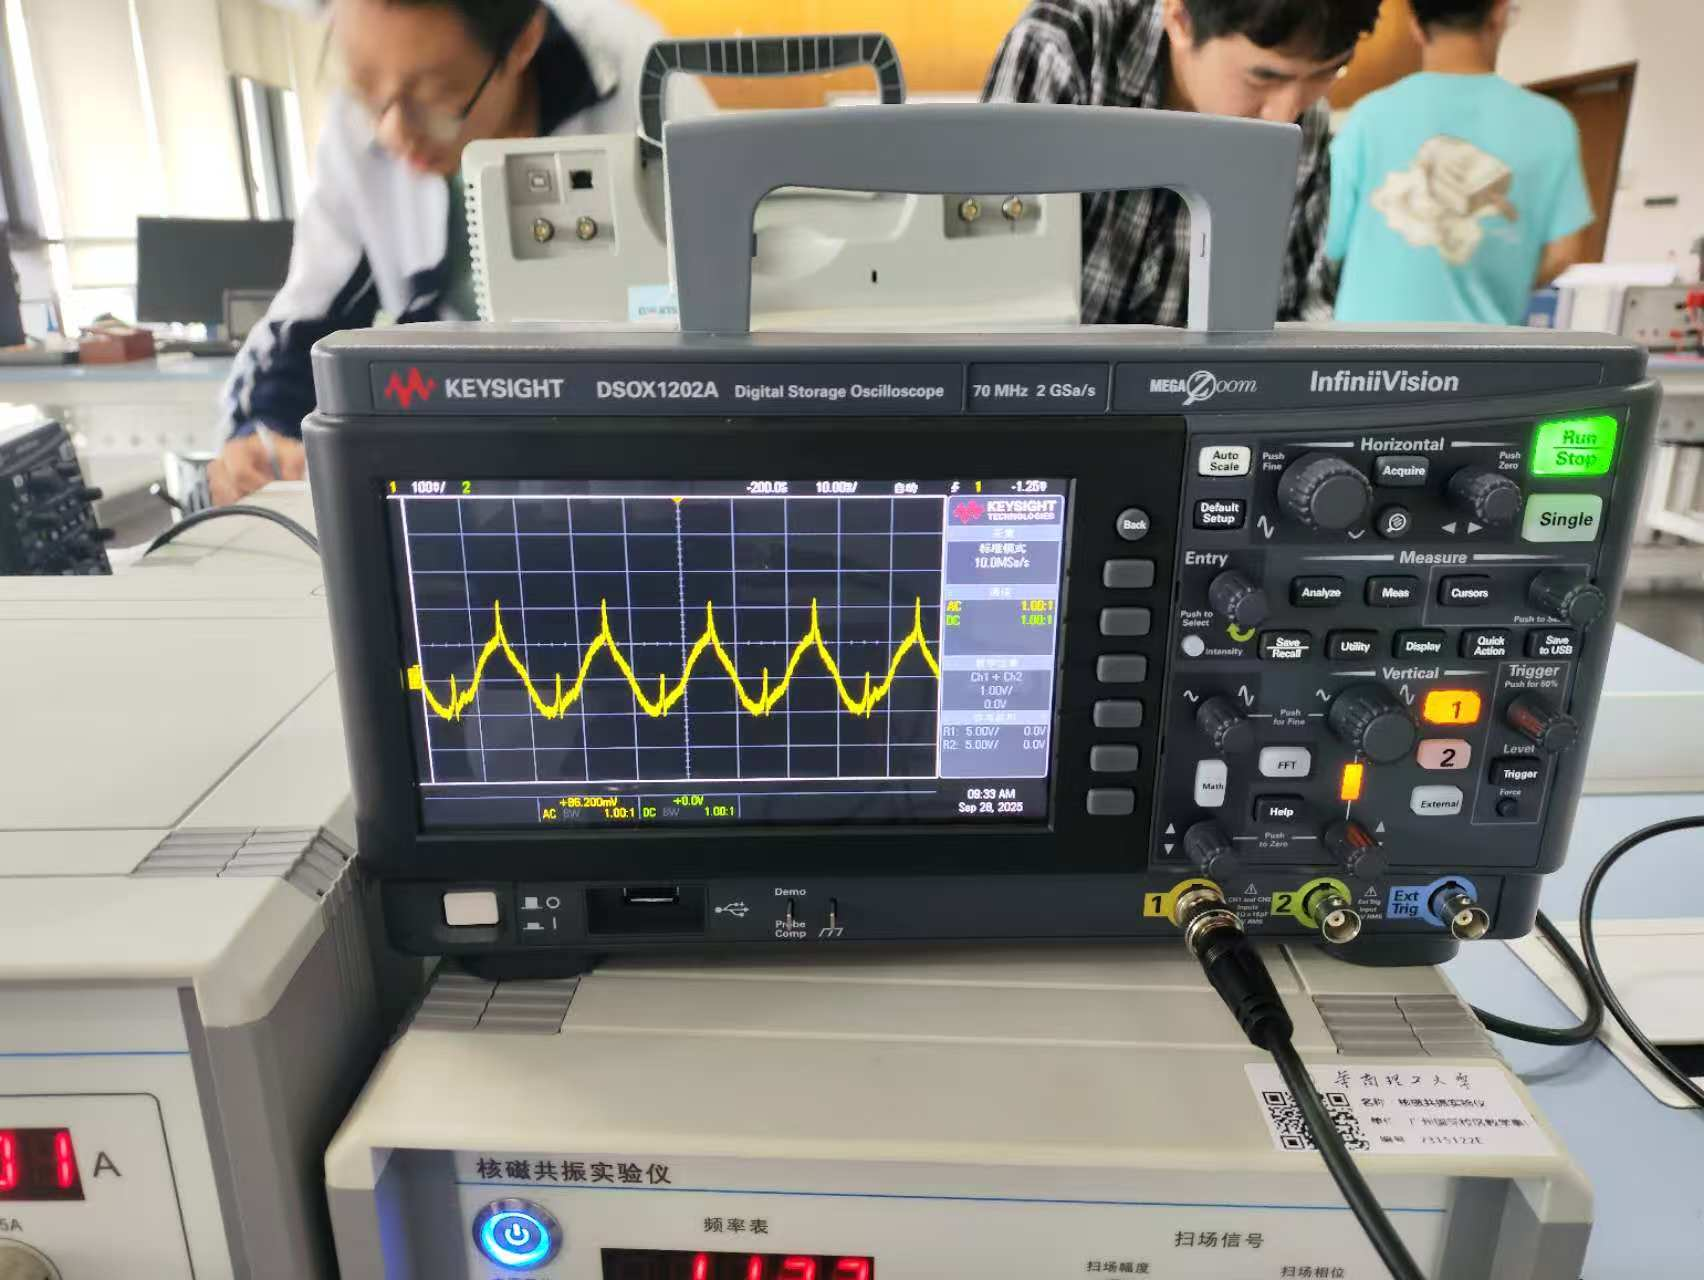
\includegraphics[width=\textwidth]{assets/硫酸铜水溶液波形.jpg}
        \caption{硫酸铜水溶液 核磁共振信号}
        \label{fig:oscilloscope}
    \end{minipage}
    \hfill
    \begin{minipage}[t]{0.48\textwidth}
        \centering
        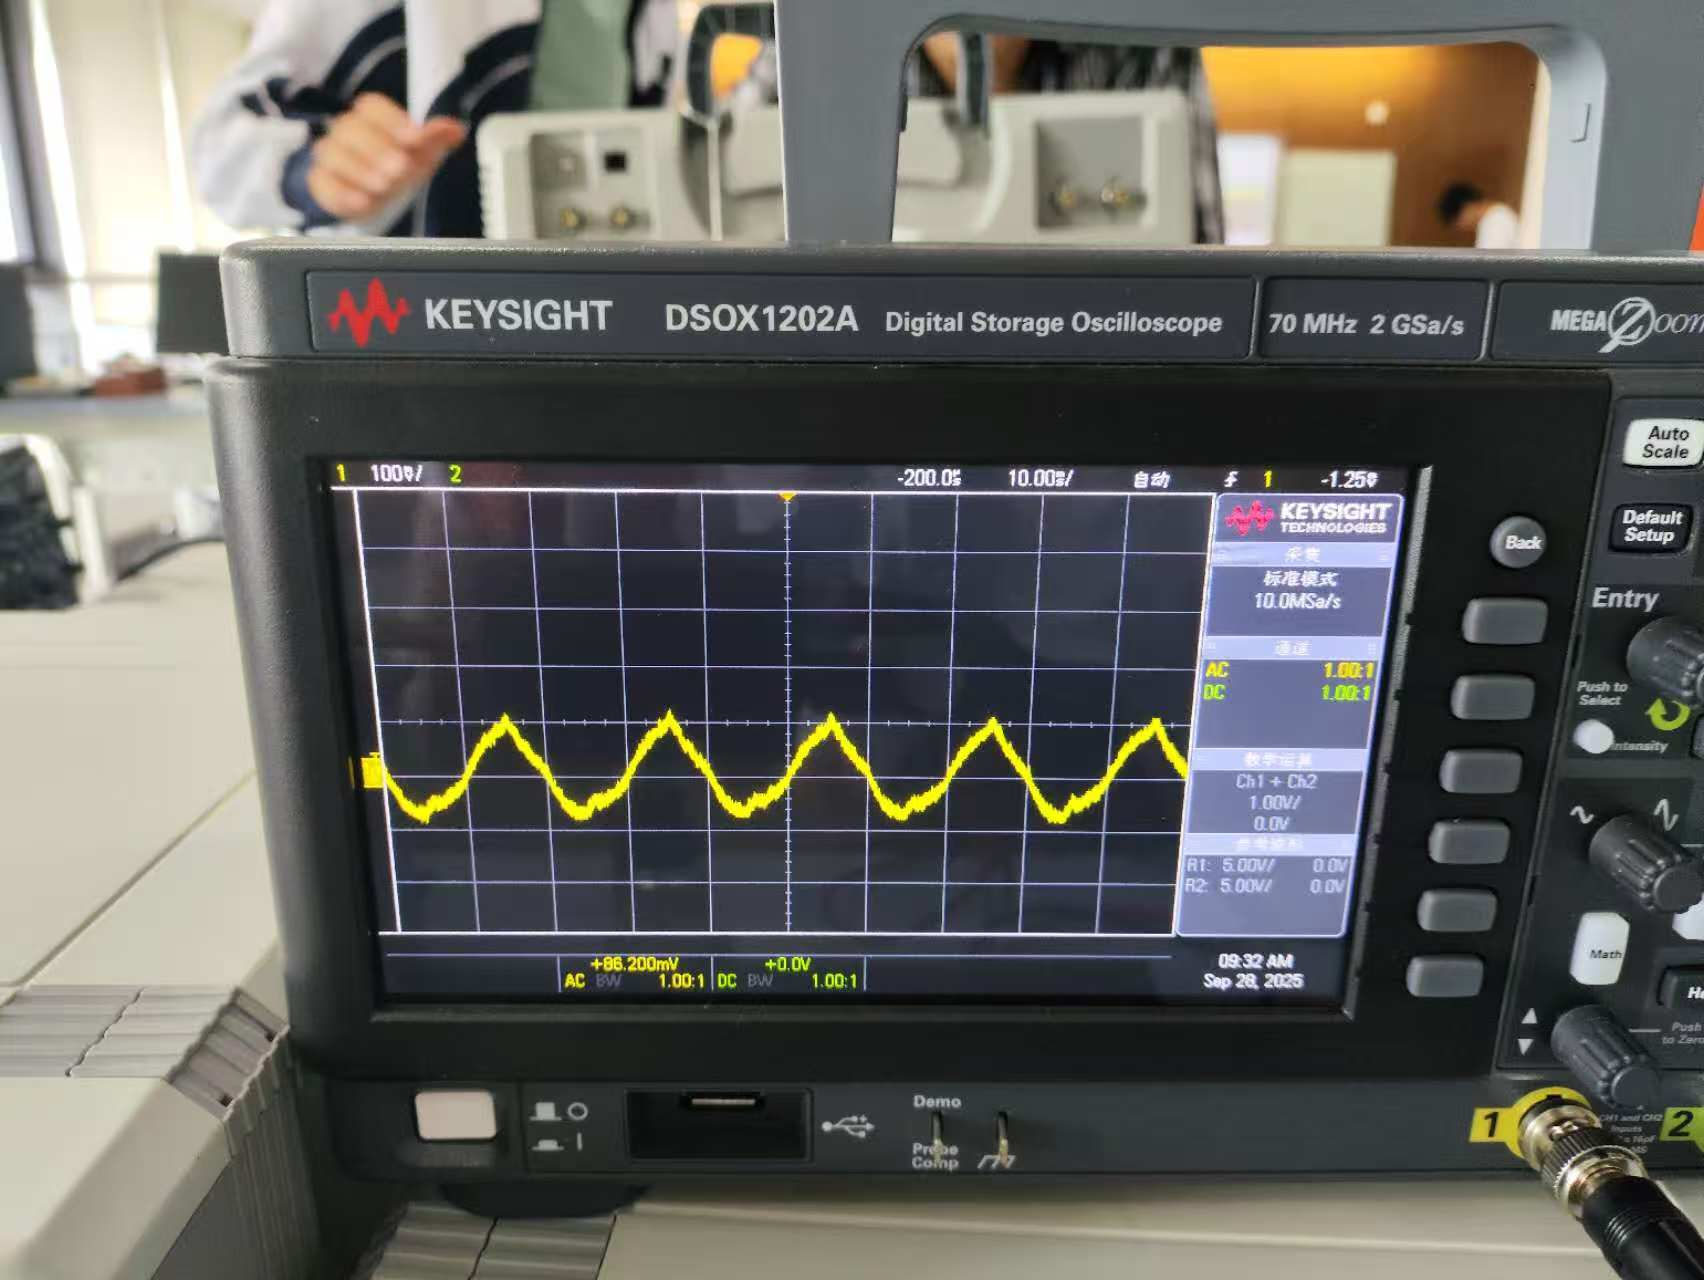
\includegraphics[width=\textwidth]{assets/聚四氟乙烯.jpg}
        \caption{聚四氟乙烯 核磁共振信号}
        \label{fig:oscilloscope2}
    \end{minipage}
\end{figure}

图\ref{fig:equipment}展示了实验过程中的仪器设置。左侧为可调直流电源，显示励磁电流为2.01A；右侧为核磁共振实验仪，显示共振频率为11.28MHz。通过精确控制这两个参数，可以实现对共振条件的精确调节，从而获得高质量的共振信号。

\begin{figure}[H]
    \centering
    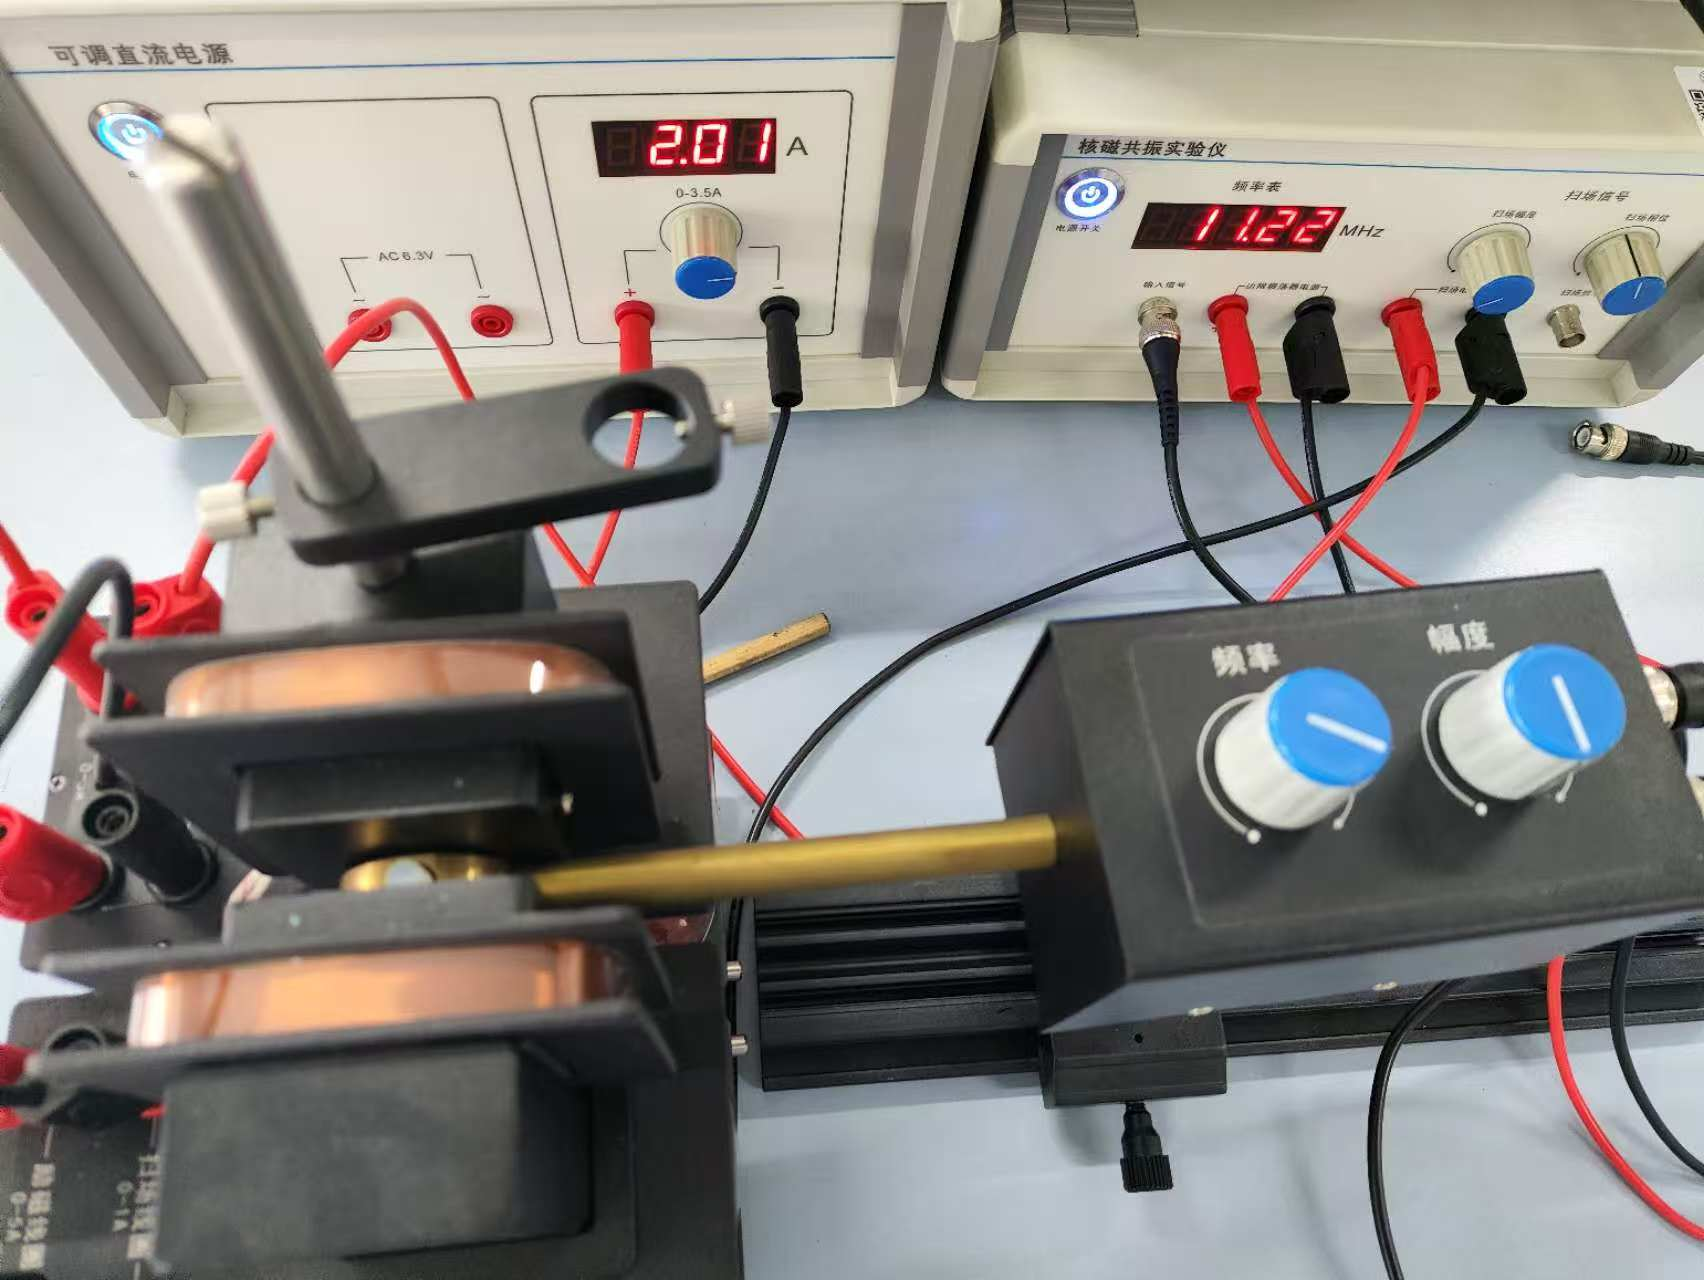
\includegraphics[width=0.8\textwidth]{assets/实验装置.jpg}
    \caption{实验仪器}
    \label{fig:equipment}
\end{figure}

图\ref{fig:test_report}展示了实验仪器的标定测试报告，提供了励磁电流与磁感应强度之间的精确对应关系，以及g因子的标准值。这些标定数据为本实验的数据处理提供了重要的参考依据。

\begin{figure}[H]
    \centering
    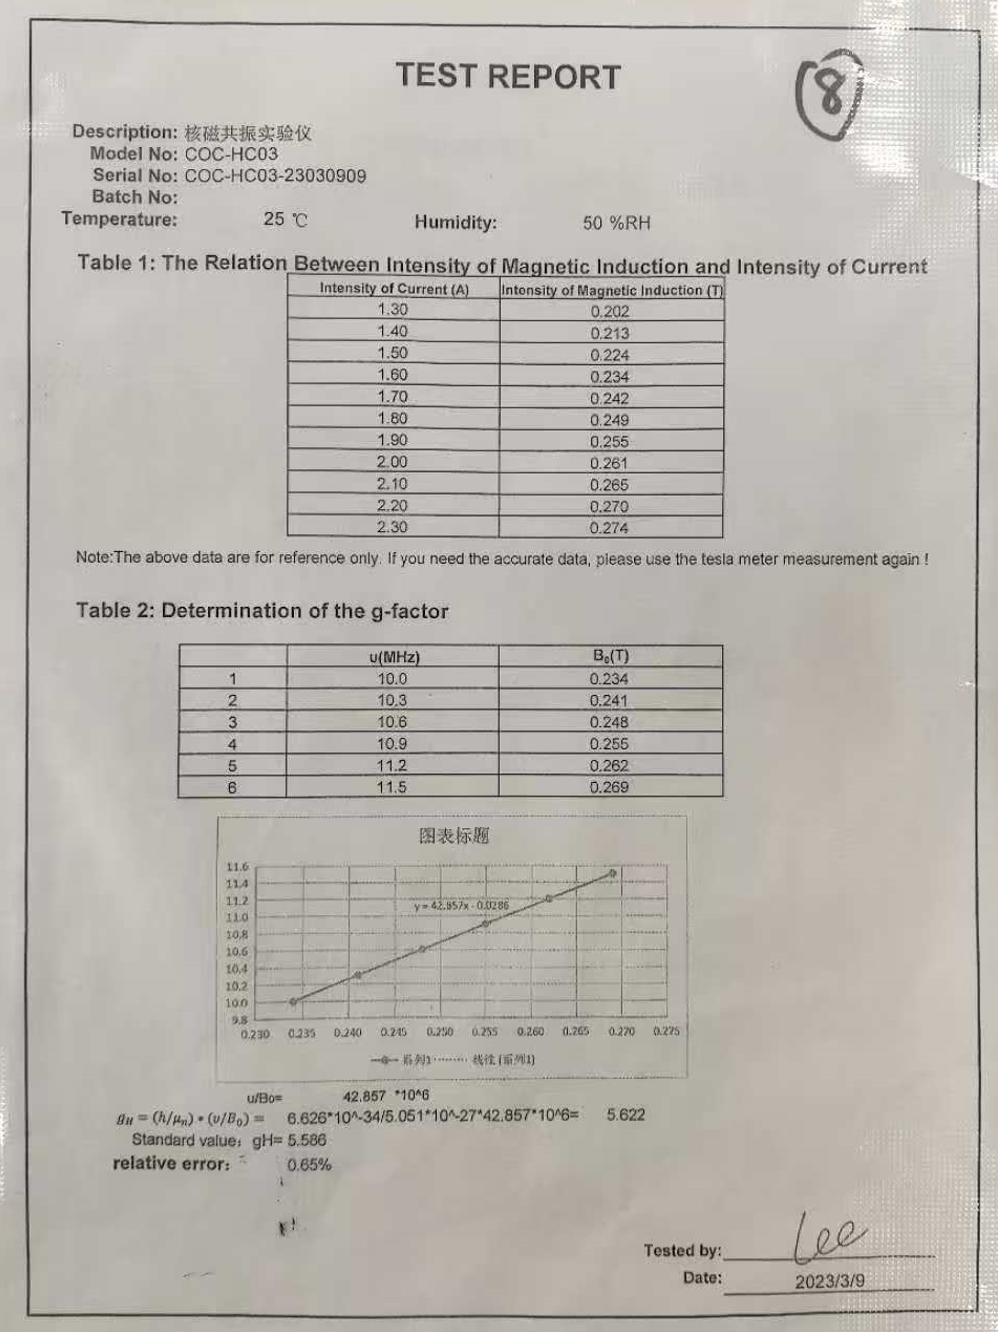
\includegraphics[width=0.6\textwidth]{assets/矫正图.png}
    \caption{实验仪器标定测试报告}
    \label{fig:test_report}
\end{figure}

\section{误差分析}

本实验的主要误差来源包括以下几个方面。首先是\textbf{磁场的不均匀性}，虽然样品被放置在磁场中心位置，但由于电磁铁结构的限制，磁场在空间上存在一定的不均匀性，这会导致样品不同位置处的原子核感受到略有差异的磁场强度，从而影响共振信号的质量和测量精度。其次是\textbf{温度的影响}，实验过程中环境温度和励磁线圈温度的微小变化会导致磁场强度的漂移，虽然实验室温度控制在25℃左右，但长时间通电后励磁线圈会发热，引起磁场的缓慢变化。第三是\textbf{频率测量的读数误差}，虽然使用了数字频率计，但在频率变化时仍存在一定的读数误差。第四是\textbf{示波器读数误差}，在判断共振信号是否等间距分布时，存在一定的主观判断误差。

对于聚四氟乙烯样品，实验中观察到前两组数据与整体线性关系偏离较大。这可能是由于在测量初期，样品位置尚未调节到最佳状态，或者磁场尚未完全稳定，导致共振条件不够理想。在后续测量中，随着样品位置的优化和磁场的稳定，数据质量明显提高，最终获得了高质量的拟合结果。

此外，样品的纯度和均匀性也会影响测量结果。虽然使用的硫酸铜溶液可以减少氢键的影响，但溶液中的铜离子可能会对局部磁场产生微小扰动。聚四氟乙烯样品的结晶度和纯度也可能影响氟核的共振特性。

尽管存在上述误差来源，但通过多次测量取平均值、仔细调节样品位置、保持环境稳定等措施，本实验获得的相对误差均小于1\%，说明实验方法和操作过程是可靠的。

\section{实验结论}

通过本次核磁共振实验，成功观察到了氢核（$^1$H）和氟核（$^{19}$F）的核磁共振现象，并测量了共振频率与磁感应强度之间的关系。实验结果表明，共振频率与磁感应强度之间存在良好的线性关系，符合核磁共振的基本理论$\nu = \frac{\gamma}{2\pi} B_0$。

对于水样品，采用过原点拟合得到的氢核磁旋比为$\gamma_H = 2.697 \times 10^8$ rad·T$^{-1}$·s$^{-1}$，与理论值的相对误差为0.82\%。对于聚四氟乙烯样品，采用过原点拟合得到的氟核磁旋比为$\gamma_F = 2.534 \times 10^8$ rad·T$^{-1}$·s$^{-1}$，与理论值的相对误差为0.63\%。这些结果验证了核磁共振理论的正确性和实验方法的可靠性。

作为对比，如果采用含截距拟合，水样品的磁旋比为$\gamma_H = 2.392 \times 10^8$ rad·T$^{-1}$·s$^{-1}$，相对误差为10.57\%；聚四氟乙烯样品的磁旋比为$\gamma_F = 2.111 \times 10^8$ rad·T$^{-1}$·s$^{-1}$，相对误差为16.18\%。这表明过原点拟合在物理意义上更为合理，尽管其相关系数可能略低。

实验过程中，通过细致调节样品位置和实验参数，成功获得了清晰稳定的共振信号。示波器上观察到的周期性共振吸收峰清晰可辨，表明实验装置工作正常，测量方法正确。通过对比不同样品的共振特性，加深了对核磁共振现象的理解，认识到不同原子核具有不同的磁旋比，这是核磁共振技术能够用于物质结构分析的物理基础。

此外，本次实验体现了数据处理的重要性。对于聚四氟乙烯样品，通过识别和剔除异常数据点，显著提高了拟合精度。这说明在实验数据分析中，需要对数据的合理性进行判断，对异常数据进行适当处理，才能获得可靠的实验结论。

核磁共振技术作为现代科学研究的重要工具，在物理学、化学、生物医学等领域具有广泛的应用价值。

\clearpage
\appendix

\section{数据处理MATLAB代码}

\begin{lstlisting}[style=Matlab-boxed,caption={核磁共振数据处理代码}]
clear; clc; close all;

%% 标定数据：电流-磁感应强度关系
I_cal = [1.30, 1.40, 1.50, 1.60, 1.70, 1.80, 1.90, 2.00, 2.10, 2.20, 2.30];
B_cal = [0.202, 0.213, 0.224, 0.234, 0.242, 0.249, 0.255, 0.261, 0.265, 0.270, 0.274];

%% 水样品数据
nu_H = [11.60, 11.23, 11.18, 10.95, 10.77, 10.30, 10.00]; % MHz
I_H = [2.24, 2.02, 2.00, 1.96, 1.80, 1.66, 1.56]; % A
% 插值得到对应的磁感应强度
B_H = [0.2716, 0.2614, 0.2600, 0.2586, 0.2490, 0.2390, 0.2290]; % T

%% 聚四氟乙烯样品数据
nu_F_all = [11.80, 11.50, 11.20, 10.90, 10.60, 10.30, 10.00, 11.65]; % MHz
I_F_all = [2.90, 2.61, 2.39, 2.17, 1.96, 1.86, 1.74, 2.77]; % A
B_F_all = [0.2980, 0.2846, 0.2746, 0.2648, 0.2570, 0.2527, 0.2448, 0.2928]; % T

% 剔除异常点（序号1、2），使用序号3-8的数据
nu_F = nu_F_all([3:7, 8]);
B_F = B_F_all([3:7, 8]);
nu_F_outliers = nu_F_all([1, 2]);
B_F_outliers = B_F_all([1, 2]);

%% 水样品线性拟合
p_H = polyfit(B_H, nu_H, 1);
nu_H_fit = polyval(p_H, B_H);
R_H = corrcoef(B_H, nu_H);
R2_H = R_H(1,2)^2;

% 水样品过原点拟合
p_H0 = polyfit([0, B_H], [0, nu_H], 1);
nu_H0_fit = polyval(p_H0, B_H);
R_H0 = corrcoef([0, B_H], [0, nu_H]);
R2_H0 = R_H0(1,2)^2;

%% 聚四氟乙烯样品线性拟合
p_F = polyfit(B_F, nu_F, 1);
B_F_range = linspace(min(B_F), max(B_F), 100);
nu_F_fit = polyval(p_F, B_F_range);
R_F = corrcoef(B_F, nu_F);
R2_F = R_F(1,2)^2;

% 聚四氟乙烯样品过原点拟合
p_F0 = polyfit([0, B_F], [0, nu_F], 1);
nu_F0_fit = polyval(p_F0, B_F);
R_F0 = corrcoef([0, B_F], [0, nu_F]);
R2_F0 = R_F0(1,2)^2;

%% 绘图：水样品
figure('Color','w', 'Position', [100, 100, 800, 600]);
plot(B_H, nu_H, 'ro', 'MarkerSize', 10, 'MarkerFaceColor', 'r', 'LineWidth', 1.5); 
hold on;
plot(B_H, nu_H_fit, 'b-', 'LineWidth', 2);
grid on;
xlabel('磁感应强度 B_0 (T)', 'FontSize', 14, 'FontWeight', 'bold');
ylabel('共振频率 \nu (MHz)', 'FontSize', 14, 'FontWeight', 'bold');
title('水样品(^1H)核磁共振频率与磁感应强度的关系', 'FontSize', 16, 'FontWeight', 'bold');
legend('实验数据', '线性拟合', 'Location', 'northwest', 'FontSize', 12);

text_str = sprintf('\\nu = %.3f B_0 + %.3f\nR^2 = %.4f', p_H(1), p_H(2), R2_H);
text(0.232, 11.4, text_str, 'FontSize', 12, 'BackgroundColor', 'w', 'EdgeColor', 'k', 'LineWidth', 1.5);

%% 绘图：聚四氟乙烯样品
figure('Color','w', 'Position', [150, 150, 800, 600]);
plot(B_F, nu_F, 'bs', 'MarkerSize', 10, 'MarkerFaceColor', 'b', 'LineWidth', 1.5); 
hold on;
plot(B_F_outliers, nu_F_outliers, 'o', 'MarkerSize', 10, 'MarkerEdgeColor', [0.5 0.5 0.5], ...
    'MarkerFaceColor', [0.8 0.8 0.8], 'LineWidth', 1.5);
plot(B_F_range, nu_F_fit, 'r-', 'LineWidth', 2);
grid on;
xlabel('磁感应强度 B_0 (T)', 'FontSize', 14, 'FontWeight', 'bold');
ylabel('共振频率 \nu (MHz)', 'FontSize', 14, 'FontWeight', 'bold');
title('聚四氟乙烯(^{19}F)核磁共振频率与磁感应强度的关系', 'FontSize', 16, 'FontWeight', 'bold');
legend('有效数据', '异常数据', '线性拟合', 'Location', 'northwest', 'FontSize', 12);

text_str = sprintf('\\nu = %.3f B_0 + %.3f\nR^2 = %.4f', p_F(1), p_F(2), R2_F);
text(0.248, 11.5, text_str, 'FontSize', 12, 'BackgroundColor', 'w', 'EdgeColor', 'k', 'LineWidth', 1.5);

%% 计算结果
fprintf('========== 水样品(^1H)结果 ==========\n');
fprintf('[过原点] 斜率 k_H0 = %.3f MHz/T\n', p_H0(1));
fprintf('[过原点] R^2 = %.4f\n', R2_H0);
gamma_H0 = 2 * pi * p_H0(1) * 1e6; % rad·T^-1·s^-1
fprintf('[过原点] 磁旋比 gamma_H0 = %.3e rad·T^-1·s^-1\n', gamma_H0);
gamma_H_theory = 2.675e8;
error_H0 = abs(gamma_H0 - gamma_H_theory) / gamma_H_theory * 100;
fprintf('理论值 gamma_H = %.3e rad·T^-1·s^-1\n', gamma_H_theory);
fprintf('[过原点] 相对误差 = %.2f%%\n\n', error_H0);

fprintf('[含截距-参考] 斜率 k_H = %.3f MHz/T, 截距 b_H = %.3f MHz\n', p_H(1), p_H(2));
fprintf('[含截距-参考] R^2 = %.4f\n', R2_H);
gamma_H = 2 * pi * p_H(1) * 1e6; % rad·T^-1·s^-1
fprintf('[含截距-参考] 磁旋比 gamma_H = %.3e rad·T^-1·s^-1\n', gamma_H);
error_H = abs(gamma_H - gamma_H_theory) / gamma_H_theory * 100;
fprintf('[含截距-参考] 相对误差 = %.2f%%\n\n', error_H);

fprintf('========== 聚四氟乙烯(^{19}F) 结果 ==========\n');
fprintf('[过原点] 斜率 k_F0 = %.3f MHz/T\n', p_F0(1));
fprintf('[过原点] R^2 = %.4f\n', R2_F0);
gamma_F0 = 2 * pi * p_F0(1) * 1e6; % rad·T^-1·s^-1
fprintf('[过原点] 磁旋比 gamma_F0 = %.3e rad·T^-1·s^-1\n', gamma_F0);
gamma_F_theory = 2.518e8;
error_F0 = abs(gamma_F0 - gamma_F_theory) / gamma_F_theory * 100;
fprintf('理论值 gamma_F = %.3e rad·T^-1·s^-1\n', gamma_F_theory);
fprintf('[过原点] 相对误差 = %.2f%%\n\n', error_F0);

fprintf('[含截距-参考] 斜率 k_F = %.3f MHz/T, 截距 b_F = %.3f MHz\n', p_F(1), p_F(2));
fprintf('[含截距-参考] R^2 = %.4f\n', R2_F);
gamma_F = 2 * pi * p_F(1) * 1e6; % rad·T^-1·s^-1
fprintf('[含截距-参考] 磁旋比 gamma_F = %.3e rad·T^-1·s^-1\n', gamma_F);
error_F = abs(gamma_F - gamma_F_theory) / gamma_F_theory * 100;
fprintf('[含截距-参考] 相对误差 = %.2f%%\n', error_F);
\end{lstlisting}

\end{document}
